	Un punto importante del presente trabajo está constituido por el módulo de interfaz entre el FPGA y la PC, ya que este es el que efectivamente logra cumplir el objetivo de proveerle al sistema la comunicación entre ambos y que cualquier dispositivo que tenga cierto grado de implementación en el FPGA, pueda transmitir y recibir datos a través del protocolo USB.\\
	
	La interfaz está constituida por el controlador USB FX2LP fabricado por Cypress Semiconducotr. Dicho controlador, es una circuito integrado que posee en su interior un microcontrolador 8051, a través del cual efectua las tareas que requiere la comunicación USB, sumado a un transceptor USB, el cual codifica y decodifica los paquetes USB que se transmiten a través del bus. A su vez, posee ciertos periféricos e interfaces que otorgan una flexibilidad que permite adecuar el chip a los requerimientos de un desarrollo determinado.\\
	
	El controlador viene montado en un circuito impreso que posee una serie de componentes adicionales que facilitan la interacción del desarrollador, tales como pulsadores, display de 7 segmentos, módulos de memoria adicional,etc. Este tipo de circuitos impresos armados con la intención de favorecer desarrollo de otros sistemas, se denomina placa de desarrollo. Una placa de desarrollo que, además, incorpora algunas herramientas extra como software, cables de conexión, fuentes, etc. toma el nombre de kit de desarrollo.\\
	
	Para este trabajo, se utiliza el kit de desarrollo CY 3684 FX2LP EZ-USB, también producto elaborado por Cypress Semiconductor. Este kit posee una placa de desarrollo como la que se observa en la Figura \ref{fig:cy3684}. Esta placa de desarrollo, posee como componente principal al controlador USB FX2LP e incorpora un display de 7 segmentos, 4 luces led multipropósito, 6 pulsadores, de los cuales 4 son de propósito general, uno de reinicio y otro que envía una señal especial para salir de un modo de bajo consumo. También tiene dos bloques de memorias EEPROM destinadas al almacenamiento del firmware (programa que ejecuta un microcontrolador), lo que otorga la posibilidad de realizar una carga no volátil de la configuración del controlador, memoria flash de \SI{64}{\kilo\byte} utilizados como RAM por el programa del controlador, un puerto USB y dos puertos UART con zócalos DE-9. Adicionalmente, cuenta con 6 puertos de 20 pines que permiten comunicarse con el controlador y 1 puerto de 40 pines, compatible con el protocolo ATA.\\
	%AQUI QUEDE
	
	
	 
	
	Como interfaz entre la FPGA y la PC se utilizó kit de de desarrollo CY3684 FX2LP EZ-USB Development Kit de Cypress Semiconductor,la que se observa en la Figura \ref{cy3684}. Esta placa posee como núcleo el controlador USB CY7C68013A, circuito integrado que posee todas las herramientas necesarias para realizar la interfaz, como así también un buen número de periféricos que permiten al desarrollador realizar pruebas y depuración.\\
	
	\begin{figure}
		\centering
		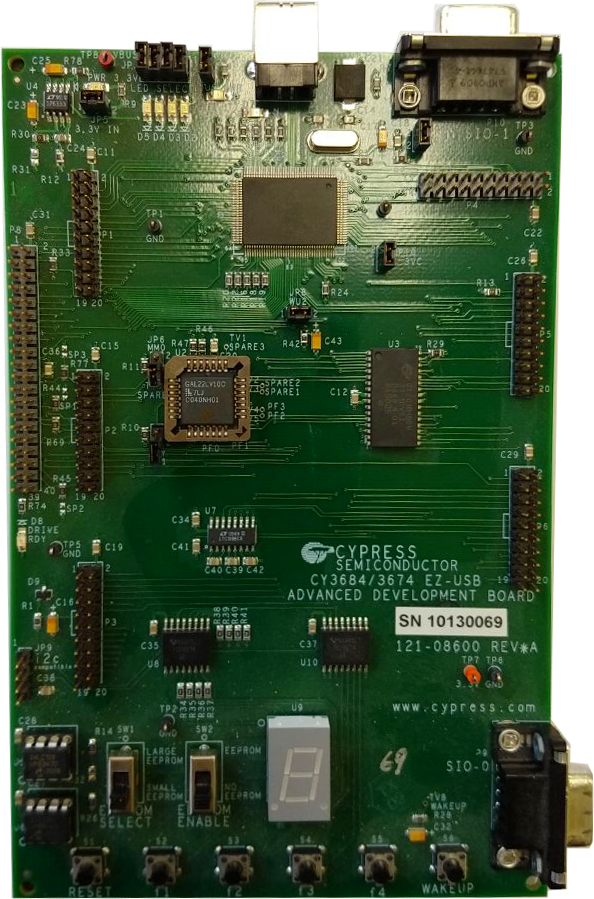
\includegraphics[width=0.4\textwidth]{32cypressboard}
		\caption{Circuito impreso principal del kit de desarrollo CY3684 FX2LP EZ-USB}
		\label{fig:cy3684}
	\end{figure}
	
	Entre estas, se destacan 6 pulsadores, de los cuales cuatro se utilizan para proposito general, uno para reestablecer los valores por defecto de la placa y uno para enviar señales de suspensión y reestablecimiento del programa actualmente cargado en el microcontrolador, lo que coloca al sistema en modo bajo consumo de energía. A su vez, posee dos memorias EEPROM que sirven para cargar firmware y archivos de configuración del sistema, un display de 8 segmentos, 4 leds de multiple propósito, dos puertos UART, una salida de pines compatible con puertos ATA y 6 puertos de 20 pines que se utilizan para la conexión hacia el chip núcleo. Como soporte para el firmware, posee también un bloque con \SI{64}{\kilo\byte} de memoria SRAM.\\
	
	Se selecciona este controlador como interfaz con el objetivo de utilizar la menor cantidad de los recursos configurables de la FPGA, de forma tal que estos queden disponibles para el desarrollo de sistemas científicos complejos que sean necesarios a posteriori.\\
	